
%(BEGIN_QUESTION)
% Copyright 2010, Tony R. Kuphaldt, released under the Creative Commons Attribution License (v 1.0)
% This means you may do almost anything with this work of mine, so long as you give me proper credit

Anta at et voltmeter viser 6 volt mellom testpunktene {\bf C} og {\bf D} når trykknappen er sluppet (ikke trykket), og også 6 volt mellom de samme punktene når trykknappen er trykket:

$$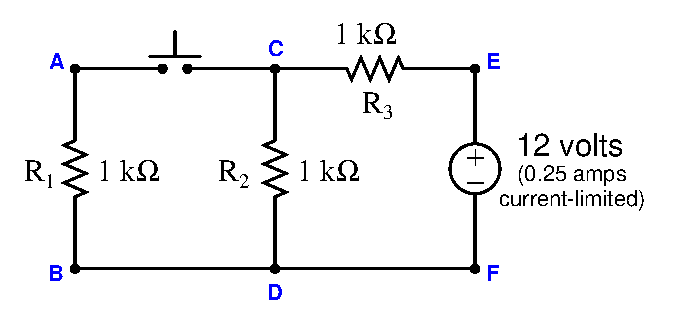
\includegraphics[width=15.5cm]{i00290x01.eps}$$

Vurder sannsynligheten for hver spesifisert feil i kretsen.  Vurder én feil av gangen (ingen samtidige feil), og avgjør om hver feil alene kan forklare {\it alle} målinger og symptomer i kretsen.

% No blank lines allowed between lines of an \halign structure!
% I use comments (%) instead, so that TeX doesn't choke.

$$\vbox{\offinterlineskip
\halign{\strut
\vrule \quad\hfil # \ \hfil & 
\vrule \quad\hfil # \ \hfil & 
\vrule \quad\hfil # \ \hfil \vrule \cr
\noalign{\hrule}
%
% First row
{\bf Feil} & {\bf Mulig} & {\bf Umulig} \cr
%
\noalign{\hrule}
%
% Another row
Bryter feilet åpen &  &  \cr
%
\noalign{\hrule}
%
% Another row
$R_1$ feilet åpen &  &  \cr
%
\noalign{\hrule}
%
% Another row
$R_2$ feilet åpen &  &  \cr
%
\noalign{\hrule}
%
% Another row
$R_3$ feilet åpen &  &  \cr
%
\noalign{\hrule}
%
% Another row
Bryter feilet kortsluttet &  &  \cr
%
\noalign{\hrule}
%
% Another row
$R_1$ feilet kortsluttet &  &  \cr
%
\noalign{\hrule}
%
% Another row
$R_2$ feilet kortsluttet &  &  \cr
%
\noalign{\hrule}
%
% Another row
$R_3$ feilet kortsluttet &  &  \cr
%
\noalign{\hrule}
%
% Another row
Spenningskilde død &  &  \cr
%
\noalign{\hrule}
} % End of \halign 
}$$ % End of \vbox

Identifiser til slutt den {\it neste} diagnostiske testen eller målingen du ville gjort.  Forklar hvordan resultatet(-ene) hjelper videre for å identifisere plassering og/eller type feil.

\vfil

\underbar{file i00290}
\eject
%(END_QUESTION)





%(BEGIN_ANSWER)

% No blank lines allowed between lines of an \halign structure!
% I use comments (%) instead, so that TeX doesn't choke.

$$\vbox{\offinterlineskip
\halign{\strut
\vrule \quad\hfil # \ \hfil & 
\vrule \quad\hfil # \ \hfil & 
\vrule \quad\hfil # \ \hfil \vrule \cr
\noalign{\hrule}
%
% First row
{\bf Feil} & {\bf Mulig} & {\bf Umulig} \cr
%
\noalign{\hrule}
%
% Another row
Bryter feilet åpen & $\surd$ &  \cr
%
\noalign{\hrule}
%
% Another row
$R_1$ feilet åpen & $\surd$ &  \cr
%
\noalign{\hrule}
%
% Another row
$R_2$ feilet åpen &  & $\surd$ \cr
%
\noalign{\hrule}
%
% Another row
$R_3$ feilet åpen &  & $\surd$ \cr
%
\noalign{\hrule}
%
% Another row
Bryter feilet kortsluttet &  & $\surd$ \cr
%
\noalign{\hrule}
%
% Another row
$R_1$ feilet kortsluttet &  & $\surd$ \cr
%
\noalign{\hrule}
%
% Another row
$R_2$ feilet kortsluttet &  & $\surd$ \cr
%
\noalign{\hrule}
%
% Another row
$R_3$ feilet kortsluttet &  & $\surd$ \cr
%
\noalign{\hrule}
%
% Another row
Spenningskilde død &  & $\surd$ \cr
%
\noalign{\hrule}
} % End of \halign 
}$$ % End of \vbox

%(END_ANSWER)





%(BEGIN_NOTES)


%INDEX% Troubleshooting review: electric circuits

%(END_NOTES)
